\chapter{Построение математической модели}
\section{Постановка задачи}
Цель работы:
\begin{itemize}
	\item Сформулировать модель математического маятника с учётом силы трения и внешних сил.
	\item Проанализировать полученную модель
	\item Провести численные эксперименты с различными параметрами, для понимания влияния на колебания маятника.
\end{itemize}

Дано:
\begin{itemize}
	\item L - длина маятника (м)
	\item g - ускорение свободного падения ($9.81 \frac{\text{м}}{\text{c}^2}$)
	\item $\theta(0) = \theta_0$ - начальный угол отклонения (рад)
	\item $\dot{\theta}(0) = \theta_1$ - начальная уголовая скорость (рад/с)
\end{itemize}
\section{Формализация}
Для вывода математической модели будем использовать полярную систему координат и второй закон Ньютона в дифференциальной форме.

Пусть сила трения пропорциональна угловой скорости маятника, а внешняя сила 
действует с периодической частотой.

\section{Построение модели}
\begin{figure}[h]  % Окружение для картинки
	\centering
	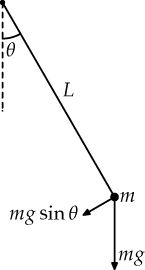
\includegraphics[height=0.3\textwidth]{imgs/pendulum_model.png}  % Вставка изображения
	\caption{Математический маятник.}  % Подпись к изображению
	\label{fig:pendulum}  % Метка для ссылки
\end{figure}

Введём полярнуюю систему координат. В качестве переменной, описывающей движение маятника, выберем угол отклонения $\theta$ от вертикали в радианах. Запишем второй закон Ньютона \cite{feinman}:
\begin{equation}
	\overrightarrow{F} = m \overrightarrow{a},
	\label{eq:2nd_Newtone}
\end{equation}
где, $\overrightarrow{F}$ - сила, приложенна к телу, $m$ - масса тела, $\overrightarrow{a}$ - ускорение тела.

Тангенциальная сила направлена по касательной к траектории движения. Сила натяжения нити не учитывается, т.к. она направлена по нормали  и не влияет на угловое движение.

Выделяя тангенциальную составляющую \cite{feinman} проекции силы тяжести ($ma_t = F_t$), получим:
\begin{equation}
	F_t = - mg\sin(\theta),
	\label{eq:F_tan}
\end{equation}
где $g$ -ускорение свободного падения.

Запишем ускорение в дифференциальной форме:
\begin{equation}
	a = \frac{dv}{dt} = \frac{d}{dt}\left(L\frac{d\theta}{dt}\right) = L \ddot{\theta}
	\label{eq:acceleration}
\end{equation}

Тогда (\ref{eq:F_tan}) , с учётом (\ref{eq:2nd_Newtone}, \ref{eq:acceleration}), можно переписать так:
\begin{equation}
	mL\ddot{\theta} = -mg\sin(\theta) \Rightarrow \ddot{\theta} +\frac{g}{L}\sin(\theta) = 0 
	\label{eq:base_model}
\end{equation}

В области малых углов $\sin(\theta) \approx \theta$.
Тогда (\ref{eq:base_model}) можно записать в виде линейной модели:
\begin{equation}
	\ddot{\theta} +\frac{g}{L}\theta = 0
	\label{eq:lin_model}
\end{equation}

Таким образом мы получили, что колебания маятника описываются обыкновенным дифференциальным уравнением. 

Обозначим $\omega^2 = \frac{g}{L}$ и добавим начальные условия для получения единственного решения. Тогда, получим системы для (\ref{eq:base_model}) и (\ref{eq:lin_model}):
\begin{equation}
	\begin{cases}
		\ddot{\theta} + \omega^2 \sin(\theta) = 0 \\
		\theta(0) = \theta_0, \ \dot{\theta}(0) = \theta_1
	\end{cases}
	\text{ или }
	\begin{cases}
		\ddot{\theta} + \omega^2 \theta = 0 \\
		\theta(0) = \theta_0, \ \dot{\theta}(0) = \theta_1
	\end{cases}.
\end{equation}

\subsection*{Модели с внешними силами}
Будем рассматривать линейную модель. Для нелинейной модели преобразования будут аналогичными.

Добавим в систему силу трения $F_{\text{тр}}$. Для простоты, пусть она будет пропорциональна скорости  изменения угла $\dot{\theta}$ с некоторым коэффициентом $\mu > 0$. Тогда модель преобразуется так: $\ddot{\theta} + \mu\dot{\theta} + \omega^2 \theta = 0 $.

На маятник может воздействовать внешняя сила, создавая вынужденные колебания: $$F_e\sin(\omega_f t),$$ где $F_e$ - амплитуда внешней силы (Н), $\omega_f$ - циклическая частота (Гц = рад/с) . Добавим эту компоненту в модель: $\ddot{\theta}  + \omega^2 \theta = F_e\sin(\omega_f t) $.

В случае, если на маятник действуют обе силы, описанные выше, то уравнение преобразуется так: $\ddot{\theta} + \mu \dot{\theta}  + \omega^2 \theta = F_e\sin(\omega_f t) $.



 
 
 
